Il problema in esame è quello di \textit{bus arbitration}, problema tipico in ambienti multi-processore. Il caso è quello in cui $n$ processori ${p_1,..,p_n}$  fanno periodiche richieste di accesso ad uno qualunque degli $m$ bus fra ${b_1,..,b_m}$. In un qualsiasi istante di tempo, un bus è assegnato al più ad un processore ed un processore sta utilizzando al più un unico bus.\\
In Figura \ref{Fig:uml} sono mostrate delle macchine a stati finiti che modellano, in prima approssimazione, il comportamento di processori e bus. Un processore invia un segnale di \textit{request} per richiedere l'accesso ad un bus. Se la richiesta ha buon fine, usa il bus fino a quando decide di rilasciarlo (segnale \textit{release}). Il controllore del bus ha un comportamento speculare: a seguito di una richiesta manda un segnale di \textit{grant} al processore, aspettando un segnale di avvenuta ricezione (\textit{ack}), e poi attende che il processore lo rilasci.\\
Rispetto alle macchine a stati di Figura \ref{Fig:uml}, si rende necessaria la realizzazione di un \textit{arbitro} che garantisca l’unicità della segnalazione di \textit{grant} per una coppia processore-bus. Inoltre l’arbitro, in un dato istante, deve poter riconoscere l’impossibilità temporanea di servire un processore e deve segnalare questa situazione al processore richiedente con un segnale di \textit{nack}.\\
Nel caso di più richieste di utilizzo di uno stesso bus da parte di processori distinti, si pone anche il problema di decidere a quale processore assegnare il bus. Vengono prese in esame due diverse politiche di gestione:
\begin{itemize}
\item Equal priority:  tutti i processori hanno la stessa priorità ed evenutali richieste in conflitto vengono servite in ordine FIFO di arrivo
\item Fixed priority:  i processori hanno una diversa priorità e in caso di richieste "simultanee" (nello stesso ciclo di clock) si serve quella del processore prioritario
\end{itemize}
\begin{center}
\begin{figure}
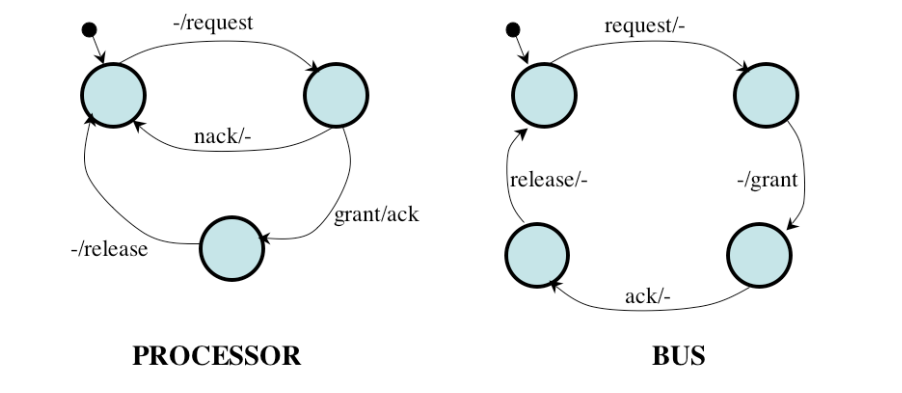
\includegraphics[scale=0.6]{uml_processor_bus}
\caption{Schemi funzionali di processori e bus}
\label{Fig:uml}
\end{figure}
\begin{figure}
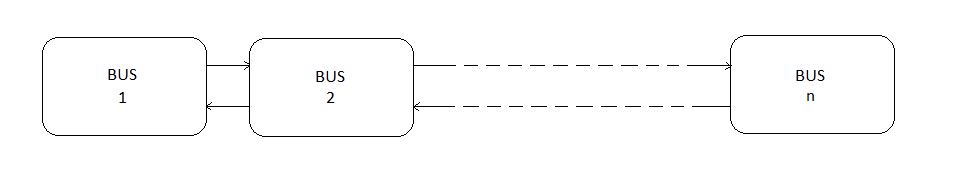
\includegraphics[scale=0.6]{2pc}
\caption{Collegamento a catena dei bus}
\label{Fig:2pc}
\end{figure}
\end{center}
Per la generazione dei segnali di \textit{grant} e \textit{nack}, l'arbitro deve far eseguire ad i nodi bus il protocollo \textit{Two-Phase Commit} in versione lineare. In questa versione del protocollo, i nodi sono collegati a catena, come in Figura \ref{Fig:2pc}. Ogni partecipante ha un numero progressivo e conosce il precedente e il successivo; l'ultimo nodo della catena sa di essere l'ultimo. Il protocollo procede attraverso due fasi successive:
\begin{itemize}
\item Fase 1: ogni nodo, partendo dal primo fino all'ultimo, comunica di essere arrivato al punto di \textit{commit} (o \textit{abort} nel caso qualcosa non abbia funzionato)
\item Fase 2: l'ultimo nodo risponde \textit{OK} e il messaggio percorre in senso inverso la catena
\end{itemize}

